\documentclass[10pt,a4paper]{article}
\usepackage{amsmath}
\usepackage{amsthm}
\usepackage{amssymb}
\usepackage{booktabs}
\usepackage{graphicx}
\usepackage{color}
\usepackage{fullpage}
\usepackage{listings}
\usepackage{color}
\usepackage{url}
\def\MakeUppercaseUnsupportedInPdfStrings{\scshape}
% for Chinese
\usepackage{fontspec} % 加這個就可以設定字體
\usepackage[BoldFont, SlantFont]{xeCJK} % 讓中英文字體分開設置
\setCJKmainfont{新細明體} % 設定中文為系統上的字型,而英文不去更動,使用原TeX\字型
\renewcommand{\baselinestretch}{1.3}

\parskip=5pt
\parindent=20pt
\footnotesep=10pt
\newtheorem{lemma}{Lemma}
\newtheorem{ques}{Question}
\newtheorem{prop}{Proposition}
\newtheorem{defn}{Definition}
\newtheorem{rmk}{Remark}
\newtheorem{note}{Note}
\newtheorem{eg}{Example}
\newtheorem{aspt}{Assumption}

\definecolor{emphOrange}{RGB}{247, 80, 0}
\definecolor{stringGray}{RGB}{109, 109, 109}
\definecolor{commentGreen}{RGB}{0, 96, 0}
\definecolor{mygreen}{rgb}{0,0.6,0}
\definecolor{mygray}{rgb}{0.5,0.5,0.5}
\definecolor{mymauve}{rgb}{0.58,0,0.82}

\lstset{
  belowcaptionskip=1\baselineskip,
  breaklines=true,
  frame=L,
%  xleftmargin=\parindent,
  language = C++,
  showstringspaces=false,
  basicstyle = \ttfamily, 
  keywordstyle = \bfseries\color{blue}, 
  emph = {symbol1, symbol2},
  emphstyle = \color{red},
  emph = {[2]symbol3, symbol4},
  emphstyle = {[2]\color{emphOrange}},
  commentstyle = \color{commentGreen}, 
  stringstyle = \color{stringGray}, 
%  backgroundcolor = \color{white}, 
%  numbers = left, % 沒有行號,複製貼上測試程式會比較方便
%  numberstyle = \normalsize, 
%	stepnumber = 1, 
%  numbersep = 10pt, 
%  title = ,
}

% "摘要", "表", "圖", "參考文獻"
\renewcommand{\abstractname}{\bf 摘要}
\renewcommand{\tablename}{表}
\renewcommand{\figurename}{圖}
\renewcommand{\refname}{\bf 參考文獻}






\begin{document}

\title{}
\author{}

%\maketitle
%\fontsize{20}{20pt}\selectfont

\begin{center}
\textbf{\Large Computer Vision Practice with Deep Learning \\[5pt]
Homework 2}

秦孝媛 R12725026 \\
資訊管理學系 一年級
\end{center}

\section*{Generic Object Detection}
\begin{enumerate}
\item (10\%) Current transformer-based object detection models are primarily developed based on DETR. However, we all know that DETR[1] has a drawback, which is slow convergence speed. Please describe why DETR series models have slow convergence speed.
\begin{itemize}
\item 造成 DETR model slow convergence speed 主要有兩個原因,第一個是「learned queries 中的 positional information,與 sinusoidal positional encoding 的方式不一致」。
\begin{figure}[hbt]
\centering
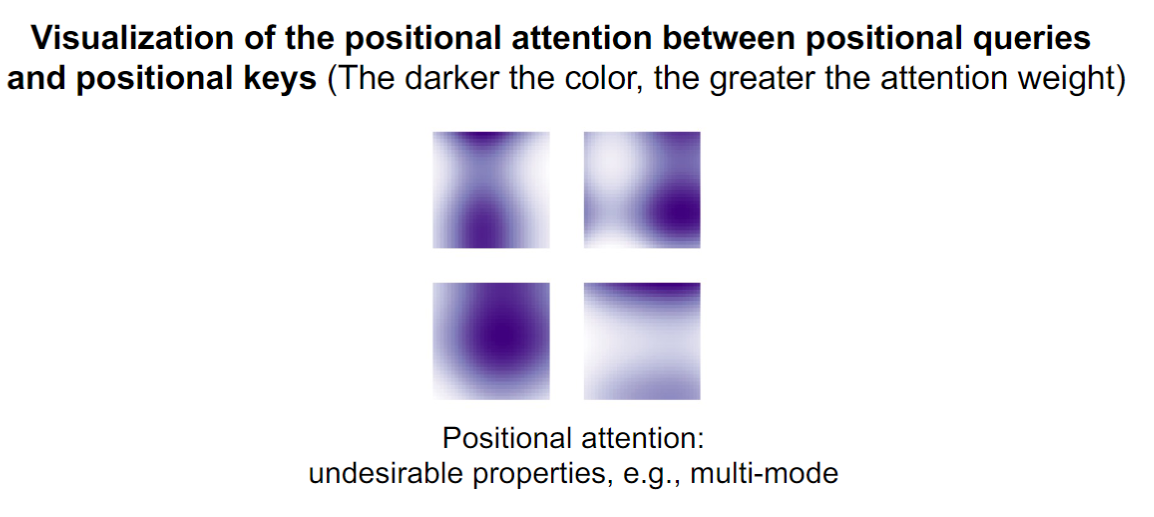
\includegraphics[width=0.8\textwidth]{DETR_slowconverge.png}
\caption{Visualization of positional attention}
\label{fig:slowConvergenceDETR}
\end{figure}
圖 \ref{fig:slowConvergenceDETR} 有 4 個 object 的 attentional map,每一個都代表了 decoder 的 learnable queries 以及 Encoder 的 positional keys 的相關性,其中顏色越黑,代表著 attention weight 越高。從這些 attentional map 中我們可以看到「multi-mode」的現象,也就是一張圖中有不只一個區域有高 attentional weight,這樣在一張圖片中有多個物體時, query 就難以快速判斷該關注哪個物體,因此導致DETR 系列 model 的 slow convergence speed。
第二個是「the discrete bipartite graph matching component」的問題,在早期訓練時,ground truth 的 distribution 是隨機分配的,導致對於同一張圖片,一個 query 時常在不同的 epochs 匹配到不同的 objects,導致 optimization 的過程變得不一致且緩慢。
\end{itemize}


\item (10\%) Two well-known papers, DAB-DETR[2] and DN-DETR[3], approach the issue of slow convergence in DETR from different viewpoints. Please describe how they address the issue.
\begin{itemize}
\item DAB-DETR:引用02-1 Generic Object Detection 一講中的內容,DAB-DETR 全名又為「Dynamic Anchor Boxes for DETR」,主要想要解決以上第一個原因(learned queries 中的 positional information,與 sinusoidal positional encoding 的方式不一致)來改善收斂速度緩慢的問題,方法是將 DETR decoder 中難解釋的 object queries,改成語意明確的 learnable anchor boxes,並動態地在每一層 layer 中更新。
\begin{figure}[hbt]
\centering
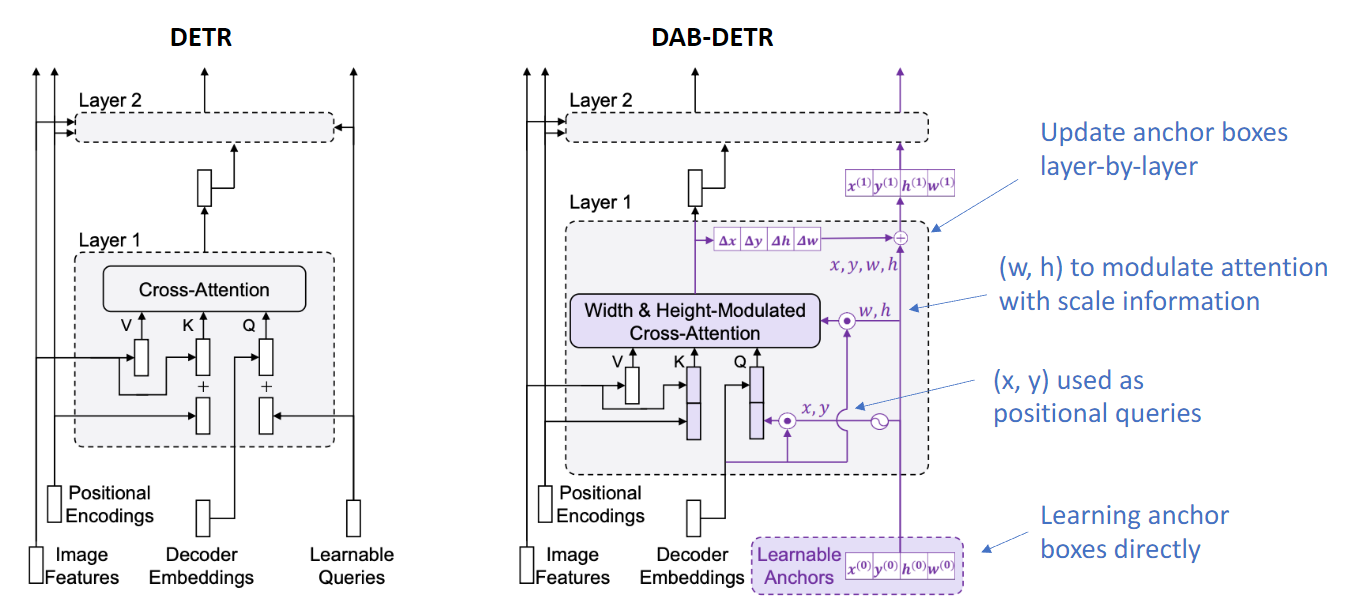
\includegraphics[width=0.8\textwidth]{DAB_DETR.png}
\caption{DAB-DETR}
\label{fig:DAB-DETR}
\end{figure}
\item DN-DETR:全名又為「DeNoising-DETR」,主要想要解決以上第二個原因(the discrete bipartite graph matching component unstable)來改善收斂速度緩慢的問題,方法是透過 query denoising,來幫助訓練過程中的 bipartite graph matching 可以穩定一些。此方法會將 noised ground truth 的 bounding box 資訊,作為 noised queries,與先前的 learnable anchor queries 一起作為 decoder 的輸入資訊。而 noised queries 不需要經過 bipartite graph matching 的過程,這樣可以幫助 DETR 減少不穩定的 bipartite graph matching component 以及快速學習到正確的 bounding box prediction。此外,因為 denoising task 中,使用的 random noise 數值通常很小,可以有效降低 optimization 的難度。


\end{itemize}
\end{enumerate}

\section*{Practical Issue 1: Knowledge Distillation}
\begin{enumerate}
\item (10\%) Briefly describe the main differences and advantages between distilled from logits and distilled from intermediate layers.
\begin{itemize}
\item 「distilled from logits」與「distilled from intermediate layers」主要的差別是,distilled from logits 會主要聚焦在 teacher model 的最後一層 output layer,而 distilled from intermediate layers 會從 intermediate layers 就去捕捉、擷取 knowledge 資訊,而不是只有最後一層 output layer 的資訊。
\item 「distilled from logits」又稱作「Response-based knowledge」,好處是容易被實作,並且因為只有需要最後一層的 output 結果,可以兼顧實際應用上隱私、安全的疑慮。在真實世界中,許多 intermediate layer 的資訊是不方便被公開使用的,因為裡面可能有牽涉個人隱私的資料或機密資料等等,在這種狀況下,如果讓每一個 layer 的內容都輕易被取得,可能會造成資安疑慮。
\item 「distilled from intermediate layers」又稱作「Feature-based knowledge」,好處是,通常相較於傳統的「Logit Distillation」會有較好的表現,因為它能夠捕捉更深層、更豐富的資訊。這種方法允許 student model 學習 teacher model 在處理資料時的中間過程,而不僅僅是最終輸出。這意味著 student model 可以獲得更多關於數據如何轉換和處理的資訊,這有助於它更好地理解和模擬 teacher model 的行為。
\item 總結來說,「distilled from logits」方法在實用性和資安上有其優勢,但在學習深度和細節上可能有限;而「distilled from intermediate layers」雖然在實現上更複雜、對資源的需求更高,但它能提供更深層次的學習和更精確的模型表現。
\end{itemize}

\item (15\%) How to perform knowledge distillation from logits? Please find a paper from the given top conference list shown in Lecture\#1 from 2021 or later discussing certain approaches performing distillation from logits and briefly describing its methodology.
\begin{itemize}
\item 如下圖 \ref{fig:Distillation_logit} 所示,傳統的 knowledge distillation from logits 即是去計算最終輸出的 distillation loss,讓 student model 可以模仿 teacher model 的預測結果。根據 Jin, Y., Wang, J., \& Lin, D. 在 2023 年的「Multi-Level Logit Distillation」論文中,將「 knowledge distillation from logits」進行進一步的改善,以提升相關表現。傳統的 「distilled from logits」通常只會進行 instance-level 的 alignment,而「distilled from intermediate layers」也只會進行 batch-level 的 alignment,但在這篇論文中,主要聚焦「final output layer logits」,並且對其進行 instance-level、batch-level 以及 class-level 的 alignment 以及 corrleation 計算,如圖 \ref{fig:Multi-Level_Logit_Distillation} 的 Multi-Level Alignment 所示,以此提升「distilled from logits」的表現。
\begin{figure}[hbt]
\centering
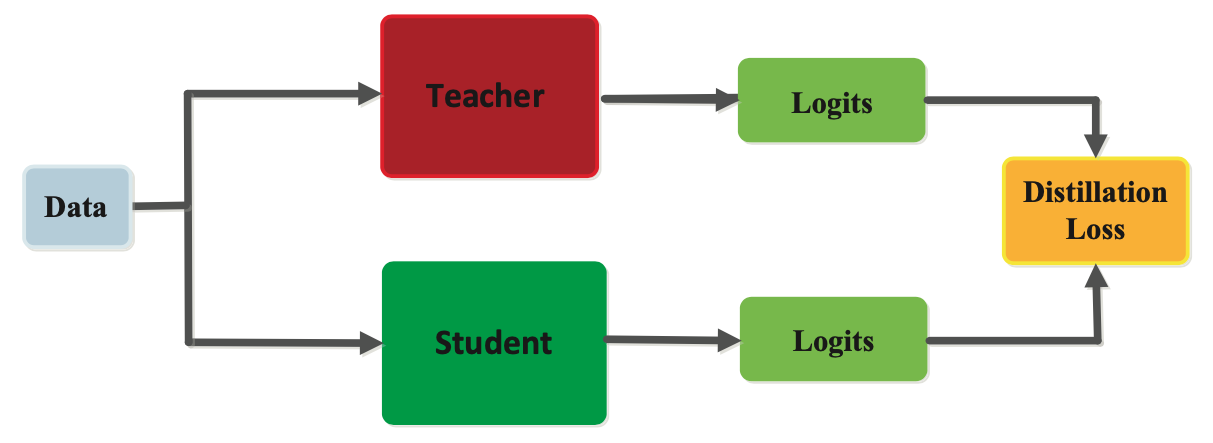
\includegraphics[width=0.8\textwidth]{Distillation_logit.png}
\caption{Distilled from logits}
\label{fig:Distillation_logit}
\end{figure}

\begin{figure}[hbt]
\centering
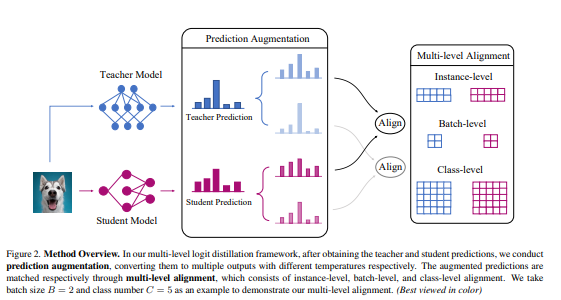
\includegraphics[width=0.8\textwidth]{Multi-Level_Logit_Distillation.png}
\caption{Multi-Level Logit Distillation}
\label{fig:Multi-Level_Logit_Distillation}
\end{figure}

%\item Jin, Y., Wang, J., & Lin, D. (2023). Multi-Level Logit Distillation. In Proceedings of the IEEE/CVF Conference on Computer Vision and Pattern Recognition (pp. 24276-24285).
\end{itemize}


\item (15\%) How to perform knowledge distillation from intermediate layers? Please find a paper from the given top conference list shown in Lecture\#1 from 2021 or later discussing certain approaches performing distillation from intermediate layers and briefly describing its methodology.
\begin{itemize}
\item 如下圖 \ref{fig:Distillation_intermediate} 所示,傳統的 knowledge distilled from intermediate layers 涉及從多個 intermediate layers 學習。在這種方法中 student model 的目標是模仿教師模型 teacher model 的 feature activations,從而達到近似的預測結果。這種 knowledge distilled from intermediate layers 的過程目標是最小化教師和學生模型之間 feature activations 的差異。在 He, R., Sun, S. 等人 2022 的「Knowledge distillation as efficient pre-training: Faster convergence, higher data-efficiency, and better transferability. 」之中,針對 feature-based knowledge distillation 加上了 non-parametric feature dimension aligning,主要是為了避免 knowledge distilled from intermediate layers 過程中可能產生的 indirect feature learning。「indirect feature learning」在此篇論文中被定義為,在 distillation 的過程中,supervision 並非直接聚焦、發生在 feature extractor 上,而是透過其他 feature extractor 之後新加上的 learnable module,這種情形會導致 feature representation learning 的過程變得緩慢且效果不佳。因此,此篇論文透過使用「singular value decomposition (SVD)」以及「power temperature scaling (PTS)」的方式,組合成更好的 aligning method,讓 student model 可以更快速、更有效地模仿 teacher model 的 feature representation。

\begin{figure}[hbt]
\centering
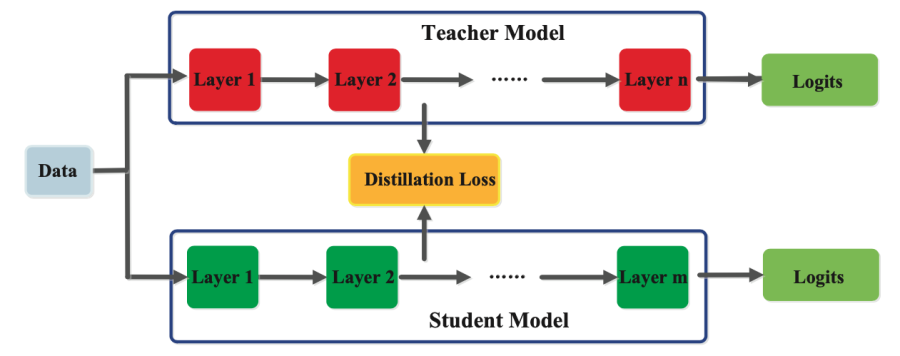
\includegraphics[width=0.8\textwidth]{Distillation_intermediate.png}
\caption{Distilled from intermediate layers}
\label{fig:Distillation_intermediate}
\end{figure}

%\item He, R., Sun, S., Yang, J., Bai, S., & Qi, X. (2022). Knowledge distillation as efficient pre-training: Faster convergence, higher data-efficiency, and better transferability. In Proceedings of the IEEE/CVF Conference on Computer Vision and Pattern Recognition (pp. 9161-9171).
\end{itemize}


\end{enumerate}

\section*{Practical Issue 2: Detecting the Novel Objects}
\begin{enumerate}
\item (20\%) CLIP[4] is a highly renowned large-scale vision-language model. It undergoes pretraining using a vast amount of paired text-image data through contrastive learning. CLIP[4] performs well on zero-shot classification task and has been the subject of further research by numerous researchers. Please describe the training process of CLIP and how it inference zero-shot classification.
\begin{itemize}
\item CLIP 的 training process 為「Contrastive pre-training」,主要是希望將 text 以及 image 映射到同一個矩陣中,根據圖 \ref{fig:Contrastive_pre_training} 所示,此模型分別針對 text 以及 image 都有一個 encoder,透過 encoder 產生 embedding 之後,將每一個 text 與 image 的 embedding 做配對,希望可以讓相對應的 text 與 image 越相似越好,而其他沒有相對應的則希望越不像越好。

\begin{figure}[hbt]
\centering
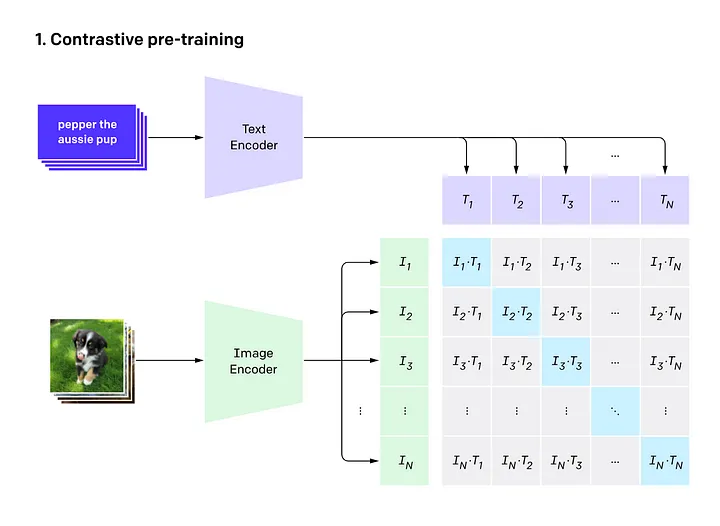
\includegraphics[width=0.8\textwidth]{contrastive_pre_training.png}
\caption{CLIP Contrastive pre-training}
\label{fig:Contrastive_pre_training}
\end{figure}


\item 關於「how it inference zero-shot classification」,如圖 \ref{fig:CLIP_inference},是在 CLIP 訓練完畢後,給定一組文字以及一張圖片,再將文字與圖片透過 encoder 映射到先前的矩陣中,觀察哪一個文字與圖片距離最相近,也就是內積最大,即可得到預測結果。
\end{itemize}

\begin{figure}[hbt]
\centering
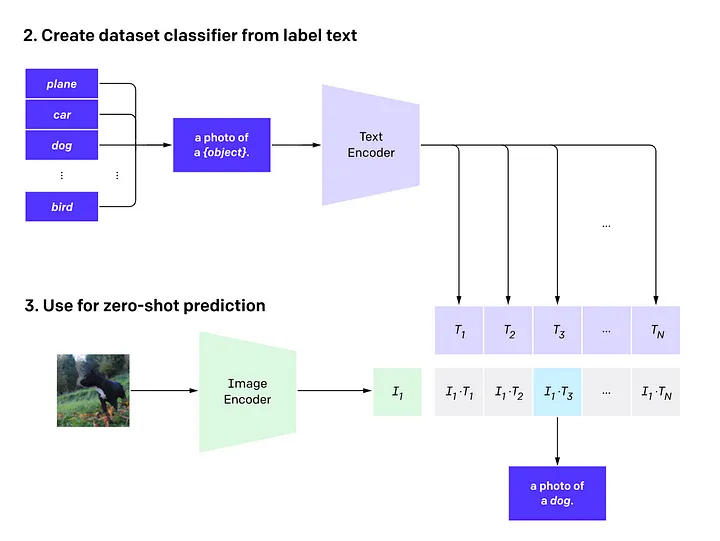
\includegraphics[width=0.8\textwidth]{CLIP_inference.png}
\caption{CLIP inference}
\label{fig:CLIP_inference}
\end{figure}


\item (20\%) In the Open-Vocabulary Object Detection task, it is intuitive to perform zero-shot classification using CLIP[4] after locating the unseen object. However, the paper RegionCLIP[5] points out that doing so presents certain challenges. Please describe these issues and explain how this paper addresses them.
\begin{itemize}
\item RegionCLIP 論文中主要提及 CLIP 雖然在 zero-shot 以及 transfer learning 的 image classification 任務中都有良好表現,但在需要辨別圖像之中的特定區域的任務,像是 object dectection 等等,就會因為 domain shift 等問題造成不佳的表現。
\item 他們解決以上問題的方法是,先從 text corpus 提取大量的 object concepts 敘述,再透過 pre-defined templates,將以上 object concepts 形成 region descriptions。接著,透過 object proposals 或是 dense sliding windows,將 image 以及其 candidate regions 放進 pre-trained CLIP 之內,為了去 align region description 以及 image regions,這樣就可以創造「pseudo labels for region-text alignment」。雖然這部分充滿雜訊,但仍然可以提供有效的資訊,使模型得以學習 region representation。最後,將「pseudo labels for region-text alignment」以及先前的「ground-truth image-text pairs」都放進 CLIP 模型中,進行原先 CLIP 的 contrastive pre-training。
\end{itemize}

\end{enumerate}
\section*{References}
\begin{itemize}

\item Generic Object Detection
\begin{enumerate}
\item Rethinking Transformer-based Set Prediction for Object Detection.Retrieved from \url{https://blog.csdn.net/xijuezhu8128/article/details/118700731}
\item Carion, N., Massa, F., Synnaeve, G., Usunier, N., Kirillov, A., \& Zagoruyko, S. (2020). End-to-end object detection with transformers. In \textit{European Conference on Computer Vision} (pp. 213-229). Springer, Cham. \url{https://link.springer.com/chapter/10.1007/978-3-030-58452-8_13}
\item Li, F., Zhang, H., Liu, S., Guo, J., Ni, L. M., \& Zhang, L. (2022). Dn-detr: Accelerate detr training by introducing query denoising. In \textit{Proceedings of the IEEE/CVF Conference on Computer Vision and Pattern Recognition} (pp. 13619-13627). \url{https://openaccess.thecvf.com/content/CVPR2022/html/Li_DN-DETR_Accelerate_DETR_Training_by_Introducing_Query_DeNoising_CVPR_2022_paper.html}
\item Liu, S., Li, F., Zhang, H., Yang, X., Qi, X., Su, H., ... \& Zhang, L. (2022). Dab-detr: Dynamic anchor boxes are better queries for detr. \textit{arXiv preprint arXiv:2201.12329}. \url{https://arxiv.org/abs/2201.12329}
\end{enumerate}

\item Practical Issue 1: Knowledge Distillation
\begin{enumerate}
\item Sundeep Teki. Knowledge Distillation: Principles, Algorithms, Applications. Retrieved from \url{https://neptune.ai/blog/knowledge-distillation}
\item Jin, Y., Wang, J., \& Lin, D. (2023). Multi-Level Logit Distillation. In \textit{Proceedings of the IEEE/CVF Conference on Computer Vision and Pattern Recognition} (pp. 24276-24285). \url{https://openaccess.thecvf.com/content/CVPR2023/html/Jin_Multi-Level_Logit_Distillation_CVPR_2023_paper.html}
\item He, R., Sun, S., Yang, J., Bai, S., \& Qi, X. (2022). Knowledge distillation as efficient pre-training: Faster convergence, higher data-efficiency, and better transferability. In \textit{Proceedings of the IEEE/CVF Conference on Computer Vision and Pattern Recognition} (pp. 9161-9171). \url{https://openaccess.thecvf.com/content/CVPR2022/html/He_Knowledge_Distillation_As_Efficient_Pre-Training_Faster_Convergence_Higher_Data-Efficiency_and_CVPR_2022_paper.html}
\end{enumerate}

\item Practical Issue 2: Detecting the Novel Objects
\begin{enumerate}
\item Radford, A., Kim, J. W., Hallacy, C., Ramesh, A., Goh, G., Agarwal, S., ... \& Sutskever, I. (2021). Learning transferable visual models from natural language supervision. In \textit{International Conference on Machine Learning} (pp. 8748-8763). PMLR. \url{https://arxiv.org/abs/2103.00020}
\item Zhong, Y., Yang, J., Zhang, P., Li, C., Codella, N., Li, L. H., ... \& Gao, J. (2022). Regionclip: Region-based language-image pretraining. In \textit{Proceedings of the IEEE/CVF Conference on Computer Vision and Pattern Recognition} (pp. 16793-16803). \url{https://openaccess.thecvf.com/content/CVPR2022/html/Zhong_RegionCLIP_Region-Based_Language-Image_Pretraining_CVPR_2022_paper.html}
\end{enumerate}

\end{itemize}



\end{document}
